\chapter{\IfLanguageName{dutch}{Stand van zaken}{State of the art}}%
\label{ch:stand-van-zaken}

\section{Inleiding}

Het onderzoek start met een uitgebreide literatuurstudie over de benodige kennis binnen het logopedisch, taal- en informatica vakdomein om geautomatiseerde en gepersonaliseerde vereenvoudigdigde teksten te verkrijgen van wetenschappelijke artikelen. Om een toepassing voor gepersonaliseerde en geautomatiseerde tekstvereenvoudiging van wetenschappelijke artikelen  op maat van deze doelgroep aan te reiken, is het van cruciaal belang om de noden van scholieren met dyslexie in de derde graad van het middelbaar onderwijs te benoemen. Het onderzoek benoemt bewezen noden met behulp van een literatuurstudie. Daarnaast moeten de problemen bij huidige wetenschappelijke artikelen ook aangekaart worden. 

\medspace

Wetenschappelijke artikelen vereenvoudigen op maat voor scholieren met dyslexie kan volgens taalexperten op verschillende manieren. Het is belangrijk om stil te staan bij de bestaande en reeds bewezen handmatige tekstvereenvoudigingstechnieken. Vervolgens komen technieken voor geautomatiseerde tekstvereenvoudiging (ATV) aan bod. Om een beter begrip te hebben op deze technieken, wordt de nodige informatie van taalverwerking met AI gegeven, alsook huidige AI-technologieën die tekstvereenvoudiging kunnen realiseren.

\medspace

AI-technologieën zijn hoogstaand en worden alsmaar robuuster, maar het is cruciaal om bij dit onderzoek aandacht te besteden aan de mogelijke problemen die AI-ontwikkelaars moeten vermijden of waarvan zij zichzelf attent op moeten maken. 

\section{Specifieke noden en richtpunten}

Om wetenschappelijke artikelen te vereenvoudigen op maat van de unieke noden van scholieren met dyslexie moet het onderzoek stilstaan bij de specifieke noden van scholieren met dyslexie in de derde graad van het middelbaar onderwijs, alsook bij de moeilijkheden bij het intensief lezen van wetenschappelijke artikelen. Deze sectie bespreekt eerst algemeen hoe scholieren met dyslexie bij het intensief lezen kunnen worden geholpen. Daarna worden de belemmeringen en moeilijkheden van wetenschappelijke artikelen aangekaart. Deze sectie beantwoordt de volgende twee onderzoeksvragen: 

\begin{itemize}
	\item Welke specifieke noden hebben scholieren met dyslexie van de derde graad middelbaar onderwijs bij het begrijpen van complexere teksten?
	\item Wat zijn de specifieke kenmerken van wetenschappelijke artikelen?
\end{itemize}

\subsection{Specifieke noden van scholieren met dyslexie in de derde graad van het middelbaar onderwijs.}

Leesvaardigheid is geen aangeboren vaardigheid, maar iets dat mensen zelf moeten aanleren \autocite{Bonte2020, VanDerMeer2022}. Hoewel dit proces vlot kan verlopen, kunnen mensen met dyslexie benadeeld worden tijdens dit proces.  Dyslexie wordt gekenmerkt door beperkt lezen en kan het voorlezen traag, radend en letter-voor-letter maken. Mensen met dyslexie kunnen tijdens het intensief lezen verschillende drempels ervaren; die worden in tabel \ref{table:dyslexia-hurdles} opgesomd.

\begin{center}
	\begin{tabular}{ | m{10cm} | m{6cm} | } 
		\hline
		\textbf{Kenmerk} & \textbf{Bron} \\ 
		\hline
		Trage woordbenoeming &  \autocite{Bonte2020} \\
		\hline
		Problemen bij het leesbegrip & \autocite{Gala2016, Bonte2020} \\ 
		\hline
		Hardnekkig letter-voor-letter lezen & \autocite{Bonte2020, Zhang2021} \\ 
		\hline
		Problemen met woordherkenning en -herinnering & \autocite{Bonte2020} \\
		\hline
		Moeite bij homofonische of pseudo-homofonische woordenschat & \autocite{bibid} \\
		\hline
		Moeite bij onregelmatige lettergreepcombinaties & \textcite{Gala2016} \\
		\hline
	\end{tabular}
	\caption{Specifieke drempels bij het intensief lezen van een tekst.}
	\label{table:dyslexia-hurdles}
\end{center}

\medspace

% TODO hoeveel percentage van de websites houdt rekening met dyslexie?

De digitalisering is de voorbije twintig jaar enkel maar in stijgende lijn en scholieren in de tweede en derde graad zijn door het gebruik van smartphones en laptops hier het meeste vatbaar op, zowel voor thuisgebruik als binnen het onderwijs. Tieners tussen 15 en 18 zijn volgens \textcite{Harvard2023} digitaal geletterd, daarom speelt de digitale weergave een essentiële rol bij een dergelijke online toepassing. Verder omschrijft dit artikel een checklist van technische elementen waaraan een webpagina of toepassing aan moet voldoen om een leesbare ervaring te voorzien voor scholieren met dyslexie. Deze noden worden weergegeven in tabel \ref{table:dyslexia-necessaries} en zijn gebaseerd op onderzoeken van \textcite{Santana2012, Harvard2023}.

\begin{center}
	\begin{tabular}{ | m{8cm} | m{8cm} | } 
		\hline
		Zachtgele, -groene of -bruine ahtergrondkleur & Consistente lay-out \\
		\hline
		Woord- en karakterspatiëring & Waarschuwingen geven omtrent formulieren, sessies (login) \\ 
		\hline
		Consistente lay-out & Duidelijk zichtbare koppen- of headingstructuur \\ 
		\hline
		Koppenstructuur &  Inhoud visueel groeperen \\
		\hline
		Huidige positie benadrukken & Duidelijke symbolen gebruiken \\
		\hline
	\end{tabular}
	\caption{Oplossingen die software-ontwikkelaars kunnen aanreiken bij een toepassing of website.}
	\label{table:dyslexia-necessaries}
\end{center}

\subsection{Specifieke kenmerken van wetenschappelijke artikelen}

Wetenschappelijke artikelen zijn van cruciaal belang voor het verspreiden van nieuwe kennis en onderzoeksresultaten, maar toch blijven ze voor velen een mysterieus en ontoegankelijk gebied vanwege de complexiteit van de inhoud en het technische jargon dat onmisbaar lijkt te zijn \autocite{Ball2017}. Dit kan het begrip van de artikelen bemoeilijken, vooral bij intensief lezen, en vormt daarmee een extra obstakel bij het gebruik van wetenschappelijke artikelen als bron van kennis tijdens de les. Wetenschappelijke artikelen volgen IMRAD, een uniform formaat voor gepubliceerde wetenschappelijke artikelen, dat bestaat uit vijf hoofdstukken: samenvatting, inleiding, methodologie, resultaten en discussie. Hoewel deze artikelen als leermiddel worden gebruikt in het middelbaar en hoger onderwijs, is de inhoud van een hoger niveau en voornamelijk gericht op mensen uit het vakgebied waarvoor het artikel is geschreven. \textcite{Pain2016, CAS2021} benadrukken de complexiteit van wetenschappelijke artikelen en de volgende aspecten waarom ze moeilijk te interpreteren zijn.

% TODO Deze artikelen betrekken jongeren met wetenschappelijk onderzoek beschreven in de methodologie en leren daarnaast een discussieerbaar en kritische vaardigheid beschreven in de discussie en conclusie. 

\medspace

\begin{center}
	\begin{tabular}{| m{4cm} | m{10cm} |}
		\hline
		\textbf{Probleem} & \textbf{Oplossing} \\
		Veel informatie in een compact formaat of \textit{high information density} & Extra uitleg schrijven bij compacte zinnen, zoals extra uitleg bij woorden of zinnen herschrijven. \\
		\hline
		Hoog gebruik van meerlettergrepige woorden & Eenvoudigere synoniemen gebruiken. \\
		\hline
		Wetenschappelijk jargon & Rekening houden met een doelgroep buiten het vakgebied door eenvoudigere synoniemen te schrijven. Indien deze niet beschikbaar zijn, kan er extra uitleg als alternatief worden gegeven. \\
		\hline
		Complexe concepten & Paragrafen herschrijven zodat ze eerst uitleg geven op een high-level niveau. Vervolgens lagen van complexiteit toevoegen om de lezer te begeleiden doorheen de methodologie, discussie en conclusie van het wetenschappelijk artikel. \\ 
		\hline
	\end{tabular}
\end{center}

\medspace

Scholieren met verschillende achtergronden hebben vaak een verschillende achtergrondkennis, wat invloed kan hebben op het tekstbegrip. Bijvoorbeeld, scholieren met een achtergrond in fysica kunnen sneller de draad oppikken bij het lezen van fysica-gerelateerde artikelen dan scholieren met een economische achtergrond. Dit maakt het moeilijk om de leesbaarheid van een tekst objectief te beoordelen, omdat jargon voor de ene groep scholieren als gemakkelijk kan worden beschouwd, terwijl het voor de andere groep juist moeilijk kan zijn. Er is dus een verschil in behoeften tussen de verschillende groepen scholieren.

\medspace

Er zijn door de jaren heen leesbaarheidsscores ontwikkeld om teksten objectief te kunnen beoordelen, aangezien ontoegankelijke en ingewikkelde zinsstructuren ook experts in het vakgebied kunnen hinderen. Er zijn twee bekende leesbaarheidsscores weergegeven in tabel \ref{table:readability-scores}. Dankzij Python-libraries, zoals Textstat\footnote{textstat} en Readability\footnote{https://pypi.org/project/readability/}, is het herschrijven van de formules niet meer nodig en bieden ze een snelle oplossing voor ontwikkelaars om een leesgraadscore te berekenen. Ook online toepassingen, zoals Textinspector, kunnen analytisch inzicht geven in de complexiteit van Engelstalige teksten. Er bestaat momenteel geen alternatief voor Nederlandstalige wetenschappelijke artikelen. Het is wel belangrijk om te benadrukken dat deze leesbaarheidsscores geen rekening houden met de achtergrondkennis van mogelijke lezers.

\begin{center}
	\begin{tabular}{ | m{6cm} | m{10cm} | } 
		\hline
		\textbf{Score} & \textbf{Uitleg} \\ 
		\hline
		Flesch Reading Ease (FRE) & Deze leesbaarheidsscore wordt berekend op zinbasis. Hoe hoger de score, hoe 'eenvoudiger' de tekst. \\
		\hline
		Gunning FOG (FOG) & Dit wordt berekend op tekstbasis. \\
		\hline
	\end{tabular}
	\label{table:readability-scores}
\end{center}

\medspace

Diverse onderzoeken van de afgelopen tien jaar wijzen uit dat wetenschappelijke teksten steeds complexer worden, wat deze teksten voor niet-experten en niet-doctoraatsstudenten ontoegankelijk maakt vanwege het gebruik van technisch jargon en ingewikkelde zinsstructuren \autocite{Ball2017, PlavenSigray2017, Jones2019}. Deze trend begon volgens onderzoek al in de tweede helft van de twintigste eeuw \autocite{Hayes1992}.

\medspace

Volgens onderzoek van \textcite{PlavenSigray2017} is de taal van wetenschappelijke artikelen de laatste jaren steeds complexer geworden. Uit een vergelijkende studie tussen abstracts en de rest van de inhoud van wetenschappelijke tijdschriften blijkt dat abstracts het meest complexe deel van een artikel vormen. De evolutie van de leesbaarheid wordt weergegeven in figuur \ref{img:fre-ndc}, waarbij de FRE- (links) en NDC-scores (rechts) getoond worden. Het onderzoek schat dat op dit moment 22\% van alle wetenschappelijke artikelen op het niveau van een masterstudent in het Engels geschreven zijn, tegenover 14\% in 1960. Deze trend is belangrijk om op te volgen in het komende decennium, omdat het een obstakel kan vormen voor toekomstige generaties.

\begin{figure}[H]
	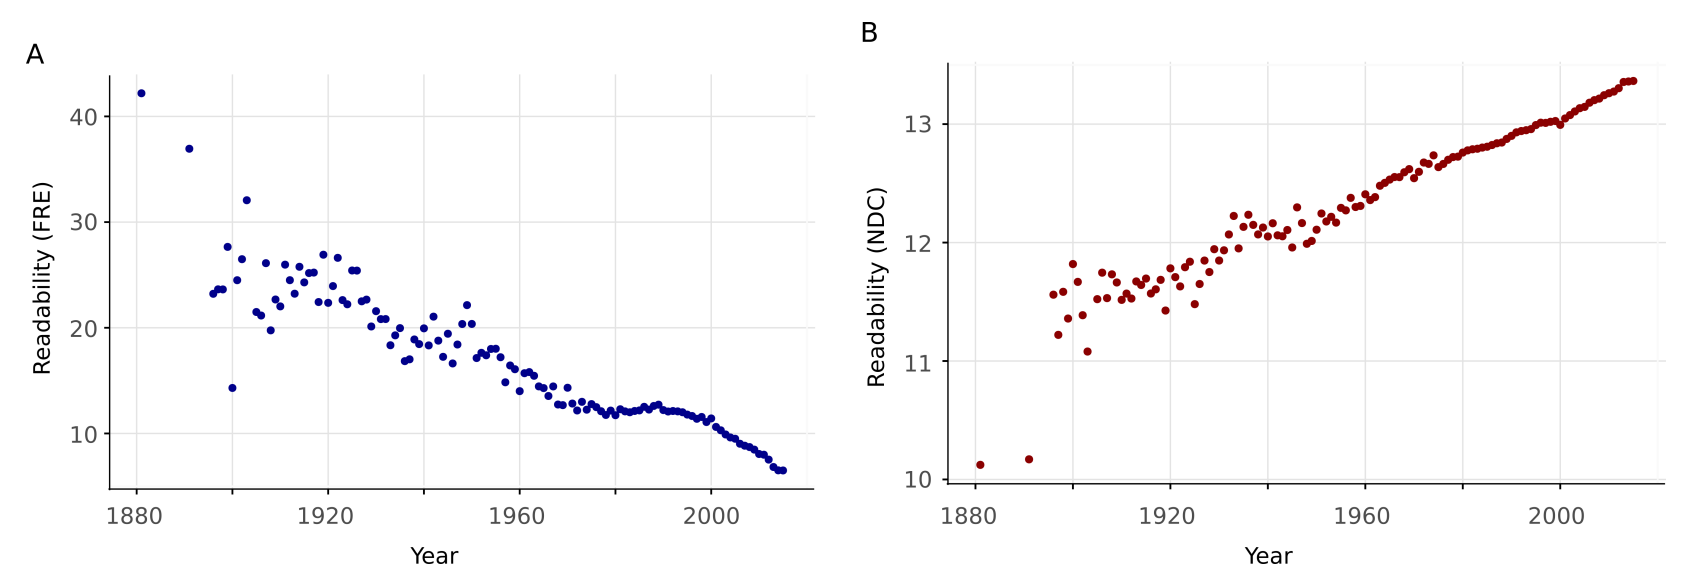
\includegraphics[width=\linewidth]{img/fre-ndc.png}
	\caption{Afbeelding uit \textcite{PlavenSigray2017}}
	\label{img:fre-ndc}
\end{figure}

\medspace

Onbegrijpelijke en ontoegankelijke zinsstructuren hinderen ook vakexperten. Zo toonde onderzoek van \textcite{McNutt2014} aan dat begrip van de methodologie en resultaten cruciaal is in het kader van reproduceerbaarheid; enkel zo kunnen wetenschappers op correcte wijze een studie reproduceren en wetenschappelijke inzichten bevestigen of met verdere resultaten verrijken. Experimenten van \textcite{Hubbard2017} wijzen namelijk uit dat het net vooral de methodologie en resultaten van een wetenschappelijk artikel zijn die een hoge leesgraad vergen. In deze context is ook het onderzoek van \textcite{Hartley1999} en \textcite{Snow2010} relevant waarin ze aantonen dat het herschrijven van abstracts de begrijpbaarheid ervan kan verhogen.

% TODO conclusie voor de noden van wetenschappelijke artikelen en noden van dyslexie


\section{Aanpakken voor tekstvereenvoudiging}
% Welke aanpakken zijn er voor geautomatiseerde tekstvereenvoudiging? 

\subsection{Manuele tekstvereenvoudiging}
% Hoe worden teksten handmatig vereenvoudigd voor scholieren met dyslexie? 

% TODO snappy inleiding

\textit{Manual text simplification} of MTS kan worden bereikt door het gebruik van eenvoudige woordenschat, zinsstructuren en formaatwijzigingen.

\begin{center}
	\begin{tabular}{ | m{2cm} | m{12cm} | } 
		\hline
		Lexicale vereenvoudiging & Moeilijke woorden vervangen door eenvoudigere synoniemen \\ 
			& Woorden- en synoniemenlijst maken \\
			& Dubbelzinnige woorden vervangen \\
			& Idiomen vervangen \\ 
			& Rekening houden met het gekende jargon van de doelgroep \\
		\hline
		Syntactische vereenvoudiging & Tangconstructies aanpassen \\
		& Zinnen langer dan negen woorden inkorten \\
		& Verwijswoorden aanpassen \\
		& Voorzetseluitdrukkingen aanpassen \\
		& Samengestelde werkwoorden aanpassen \\
		& Actieve stem gebruiken \\
		& Onregelmatige werkwoorden vermijden \\
		\hline
		Formaataanpassingen & Marges aanpassen \\
		& Lettertype en -grootte aanpassen \\
		& Woord- en karakterspatiëring aanpassen \\
		& Herschrijven en -structureren als opsomming of tabelvorm \\
		& \\
		\hline
	\end{tabular}
	\label{table:manual-simplification}
\end{center}

\medspace

Volgens \textcite{Hollenkamp2020} en \textcite{McCombes2022} moeten vereenvoudigde of samengevatte wetenschappelijke artikelen drie vragen kunnen beantwoorden: waarom werd het onderzoek uitgevoerd, wat zijn de experimenten en wat zijn de conclusies van de onderzoekers? Dit omvat de achtergrondinformatie, hypotheses, methoden, resultaten, implicaties, beperkingen en aanbevelingen. Om de tekst begrijpelijker te maken, kan deze worden omgezet in een ander formaat, zoals post-it notes, tabelvorm of opsommingen \autocite{Rijkhoff2022}. 

\subsection{Bevoordelende effecten van MTS bij scholieren met dyslexie}

Onderzoek toont aan dat vereenvoudigde teksten het leesbegrip en woordherkenning van kinderen met dyslexie significant kunnen verbeteren \autocite{RiveroContreras2021}. Bovendien blijkt uit experimenten dat frequent woordgebruik de ontcijfertijd bij mensen met dyslexie significant vermindert, en dat teksten met verminderde lexicale complexiteit minder leesfouten opleveren voor mensen met dyslexie \autocite{Rello2013a, Gala2016}. Deze studies benadrukken ook moeilijkheden van kinderen met dyslexie bij het lezen van woorden met onregelmatige lettergreepcombinaties. Mensen zonder dyslexie bereiken doelwaarden onder optimale omstandigheden, zoals aangegeven door de richting van de pijl op figuur \ref{img:readability-mean-fixation-duration}. Het gebruik van veelvoorkomende woorden vermindert de decodeertijd en verbetert het leesbegrip voor mensen met dyslexie.

\medspace

\begin{figure}
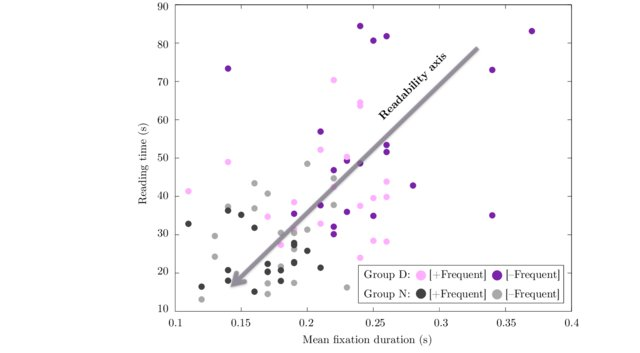
\includegraphics[width=\linewidth]{img/readability-mean-fixation-duration.png}
\caption{Afbeelding van \textcite{Rello2013a}}
\label{img:readability-mean-fixation-duration}
\end{figure}

\medspace

Er is weinig onderzoek gedaan naar de effecten van syntactische vereenvoudiging op kinderen en scholieren met dyslexie. In het experiment van \textcite{Linderholm2000} had het aanpassen van causale structuren een significant effect op het leesbegrip en de foutenmarge van de bevraagden met een lage leesgraad. Door coherentieonderbrekingen te herstellen en tekstgebeurtenissen in een tijdsafhankelijke volgorde te plaatsen, konden zowel vaardige als minder vaardige lezers profiteren van de revisies. Verbaal parafraseren had geen significant effect op lezers met dyslexie, volgens \textcite{Rello2013c}. De bevraagden waren tussen de 13 en 37 jaar oud, met een gemiddelde leeftijd van 21 jaar. Het tekstformaat bleef ongewijzigd, maar lettertypes werden aangepast.

\medspace

Volgens onderzoek van \textcite{Nandhini2013} kan het personaliseren van samenvattingen de leesbaarheid van scholieren met dyslexie verbeteren. Het experiment maakt gebruik van onaangepaste zinnen uit de oorspronkelijke tekst die op maat van de lezer zijn gepresenteerd en herstructureert deze volgens de oorspronkelijke tekst. Door de belangrijkste zinnen onaangepast te laten en de structuur aan te passen, wordt de tekst toegankelijker gemaakt voor de lezer. Hoewel de resulterende logische structuur door de onderzoekers in twijfel werd getrokken, was de leesbaarheid van de deelnemers significant beter dan bij de oorspronkelijke tekst, zonder negatieve effecten op het leesbegrip.

\medspace

Onderzoeken hebben aangetoond dat scholieren met dyslexie gevoeliger zijn voor veranderingen in visuele parameters, zoals lettertype, karakterafstand, tekst- en achtergrondkleur en grijswaarden. Om de leesbaarheid te verbeteren, worden minimalistische ontwerpen met pictogrammen en afbeeldingen aanbevolen, evenals lettergrootte groter dan 14pt en een sans-serif, monospaced of roman lettertype. Volgens \textcite{Rello2015, Bezem2016, Rello2017} zijn lichtgrijze achtergronden met zwart lettertype op een gele achtergrond, of zachtgele, -groene of lichtblauwe achtergrondkleuren de beste kleurencombinaties. Het gebruik van lettertypen zoals OpenDys heeft geen effect op lezers met of zonder dyslexie, terwijl cursieve lettertypen worden afgeraden, aldus \textcite{Rello2013b, Rello2015}.

\medspace

Conclusie. In tabel \ref{table:benefits-mts} worden de bewezen technologieën opgesomd met hun samenhangend voordeel.

\medspace

\begin{center}
	\begin{tabular}{ | m{6cm} | m{6cm} | } 
	\hline
	\textbf{Techniek} & \textbf{Bewezen voordeel} \\
	\hline
	Frequent woordgebruik & Lagere decodeertijd \\
	& Beter leesbegrip \\
	\hline	
	Verwerpen van onregelmatige lettergrepen & Verminderde decodeertijd \\
	& Beter leesbegrip \\	
	\hline
	Causale structuren aanpassen & Beter leesbegrip \\
	& Minder fouten bij het intensief lezen \\
	\hline	
	Tekstgebeurtenissen in een tijdsafhankelijke volgorde plaatsen & Beter leesbegrip bij het reviseren \\
	\hline
	Coherentieonderbrekingen herstellen & Beter leesbegrip bij het reviseren \\
	\hline
	Gepersonaliseerde samenvatting & Betere leesbaarheid \\
	\hline
	Zachtkleurige achtergrond & Betere leesbaarheid \\
	\hline
	Niet-cursieve, sans-serif lettertypen & Betere leesbaarheid \\
	\hline
	Lettertype groter dan 14pt & Betere leesbaarheid \\
	\hline
	\caption{Bewezen voordelen van MTS op mensen met dyslexie.}
	\label{table:benefits-mts}
	\end{tabular}
\end{center}

\subsection{Aanpak voor ATV.}
% Welke toepassingen, tools en modellen zijn er beschikbaar om Nederlandse geautomatiseerde tekstvereenvoudiging met AI mogelijk te maken? 

Tekstvereenvoudiging is het proces waarbij het technische leesniveau en het woordgebruik van een geschreven tekst wordt verminderd. Dit leidt tot een betere leeservaring zonder het verlies van de kerninhoud tijdens het lezen van de tekst. Met de laatste evolutie in machinaal leraren is dit een proces dat geautomatiseerd kan worden. \textit{Automatic text simplification} of ATS is een onderdeel van natuurlijke taalverwerking binnen machinaal leren (ML). Dit omvat verschillende technieken zoals tekstanalyse, taalherkenning, -generatie, spraakherkenning en -synthese, en semantische analyse. NLP stelt computers in staat om menselijke taal te begrijpen en te communiceren op een natuurlijke manier. 

\medspace

De begrippen die volgen worden behandeld in \textcite{Sohom2019, Eisenstein2019} en zijn cruciaal voor de daaropvolgende concepten.

\medspace

Er zijn vier manieren om tokens in een tekst te splitsen en zo een woordenschat op te bouwen, namelijk op woord-, karakter-, subwoord- en zinniveau, volgens onderzoek van \textcite{Menzli2023}. Bij karakter-tokenisatie neemt de inputlengte toe, maar heeft volgens \textcite{Ribeiro2018} weinig bruikbare use cases. Het opsplitsen van zeldzame woorden in kleinere stukken om een woordenschat op te bouwen biedt voordelen ten opzichte van tokenisatie op woordniveau, aldus \autocite{Iredale2022}.

\medspace

In NLP is het lemmatiseren gebaseerd op stemming, maar het houdt ook rekening met de betekenis van elk woord. Er zijn Nederlandstalige modellen beschikbaar voor lemmatiseren, zoals JohnSnow\footnote{https://nlp.johnsnowlabs.com/2020/05/03/lemma\_nl.html}. Bij omgekeerd lemmatiseren wordt een afgeleide van de stam bepaald, bijvoorbeeld enkelvoud of meervoud voor zelfstandige naamwoorden zoals 'hond' \autocite{Eisenstein2019}. Bij het parseren krijgt elk woord of zinsdeel een label toegewezen, zoals zelfstandig naamwoord, bijwoord, werkwoord, bijzin of stopwoord. Het identificeren van zinsdelen wordt 'chunking' genoemd. Parsing heeft een ambiguïteitsprobleem omdat bijvoorbeeld een 'plant' niet gelijk is aan de vervoeging van het werkwoord 'planten' \autocite{Eisenstein2019}.

\medspace

Om de betekenis van elk woord in een tekst te begrijpen, moet een machine in staat zijn om de betekenis achter elk token te begrijpen. Dit is waar \textit{sequence labeling} om de hoek komt kijken, volgens \textcite{Eisenstein2019}. Elk woord in een tekst wordt gekoppeld aan een label voor \textit{Part-of-Speech} (PoS) of \textit{Named-Entity-Recognition} (NER). Deze fase van NLP achterhaalt de structuur van een tekst. PoS-tagging richt zich op de grammaticale categorieën van woorden, terwijl NER-labeling zich richt op het herkennen van specifieke entiteiten in een tekst. Bij PoS-tagging worden de woorden in een zin geanalyseerd. Elk woord wordt gekoppeld aan een grammaticale categorie, zoals een zelfstandig naamwoord, werkwoord, bijvoeglijk naamwoord of bijwoord. \textit{PoS-tagging} helpt bij het begrijpen van de syntactische structuur van een zin en is nuttig bij parsing en machinevertaling. Een voorbeeld van PoS-tagging is te zien in figuur \ref{fig:pos-labeling} en is afkomstig uit \textcite{Bilisci2021}.

\begin{figure}[H]
	\begin{center}
		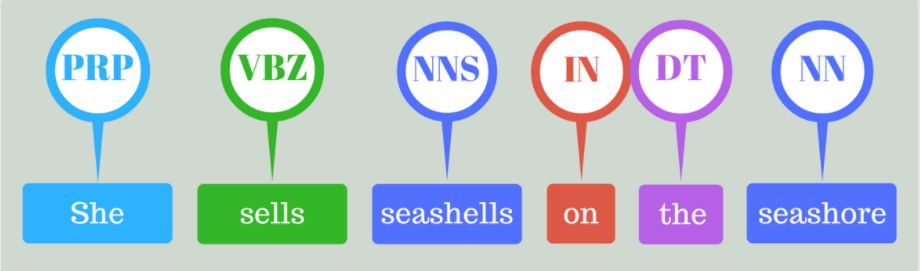
\includegraphics[width=10cm]{img/poslabeling.png}
	\end{center}
	\caption{Voorbeeld van PoS-labeling. }
	\label{fig:pos-labeling}
\end{figure}

\medspace

NER-labeling wordt gebruikt om namen van personen, organisaties en locaties te herkennen en te classificeren. Het is een techniek om specifieke informatie uit tekst te halen, zoals het identificeren van de namen van personen, plaatsen of bedrijven die in nieuwsartikelen worden genoemd, of het extraheren van belangrijke data of getallen uit financiële rapporten, aldus \textcite{Jurafsky2014}. Figuur \ref{fig:ner} illustreert deze taak. Er zijn vier verschillende vormen van NER-labeling, zoals beschreven door \textcite{Li2018}: \textit{dictionary-based}, \textit{rule-based}, \textit{ML-based} en \textit{deep learning-based}. De eerste twee maken gebruik van vooraf gedefinieerde woordenboeken en regels, terwijl de laatste twee gebruik maken van statistische of neurale netwerken om te leren hoe entiteiten te herkennen. Elke vorm maakt gebruik van verschillende kenmerken en representaties om entiteiten te modelleren. \textcite{Poel2008} heeft een neurale netwerkmodel onderzocht voor PoS-tagging van Nederlandstalige teksten. Het model behaalde een nauwkeurigheid van 97,88\% voor bekende woorden en 41,67\% voor onbekende woorden en maakte gebruik van de Corpus Gesproken Nederlands (CGN) als trainingsdata. In de verwerking van tekst maken NLP-systemen gebruik van embeddings om woorden numeriek te representeren. Traditionele word embeddings bouwen een woordenschat op zonder de betekenis ervan in context te begrijpen. Contextuele word embeddings begrijpen daarentegen wel de context van een woord \autocite{Eisenstein2019}. 

\subsection{Prompt engineering}

Large Language Models of LLM's genereren tekst en karakters op basis van de waarschijnlijke uitkomst van een gegeven input. De meest gekende LLM's zijn GPT-3, BERT en T5 en dienen regelmatig als de fundering voor ge-fine-tunede modellen. Deze modellen maken gebruik van een neuraal netwerk om patronen in de input te herkennen en deze patronen te gebruiken om voorspellingen te doen over de uitvoer \autocite{Liu2020}. Iedereen kan volgens \textcite{McFarland2023} een input of prompt schrijven. Deze tools zoals chatbots zijn ontworpen om zo intuïtief mogelijk te zijn voor een algemeen doelpubliek. Prompt engineering is een steeds belangrijkere vaardigheid die nodig is om effectief te communiceren met LLM’s, zoals ChatGPT \autocite{Harwell2023}. Deze vaardigheid wordt geïllustreerd in \ref{img:prompt-engineering}.

\begin{figure}[H]
	\begin{center}
		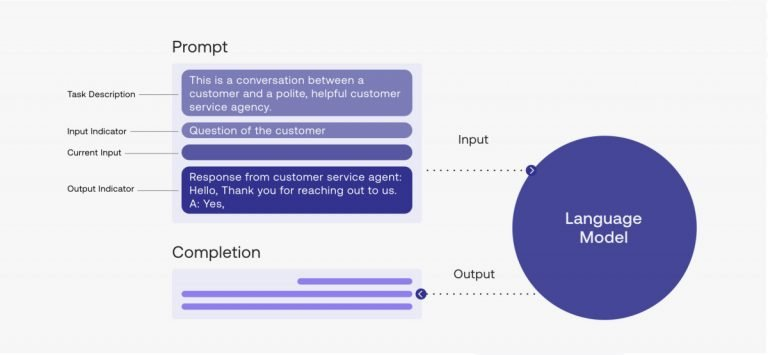
\includegraphics[width=8cm]{img/prompt-engineering-medium.png}
	\end{center}
	\caption{Afbeelding uit \textcite{McFarland2023}}
	\label{img:prompt-engineering}
\end{figure}

Deze prompts kunnen volgens \textcite{Liu2020} gebruikt worden om werk te produceren dat is aangepast aan het doel. Een concrete en geoptimaliseerde prompt omvat een concrete scope, duidelijke vraagstelling, specifieke sleutelwoorden, de context en ten slotte gepersonaliseerde keuzes \autocite{McFarland2023}. Bij een zoekopdracht moeten voldoende parameters in de prompt worden opgenomen. Zo niet zal het model te algemeen blijven en mogelijks afwijken van de intentie van de gebruiker. Effectieve AI prompt engineering leidt tot hoogwaardige trainingsgegevens die het AI-model in staat stellen om nauwkeurige voorspellingen en beslissingen te maken \autocite{Liu2020}. 

\medspace

Prompt patterns is samen met prompt engineering naar boven gekomen en is vergelijkbaar met software patterns. Deze patronen zijn herbruikbare oplossingen voor veelvoorkomende problemen in een bepaalde context, waaronder vooral de interactie bij het werken met LLM's. \textcite{White2023} benoemt vier \textit{prompt patterns}:

\begin{itemize}
	\item	Intent-prompts waarbij een LLM een instructie krijgt met een specfiek verwacht antwoord.
	\item	Restriction-prompts die het antwoord van een LLM inperkt. Deze pattern is noodzakelijk om een LLM binnen de lijnen te houden.
	\item 	Contextualization-prompts verzekeren dat de output van een LLM relevant is. Een context wordt aan de LLM meegegeven.
	\item	Expansion/reduction-prompts genereren een beknopte output met voldoende details. 
\end{itemize}

\section{De verschillende soorten ATS}

Tekstvereenvoudiging kan bijdragen aan het begrijpen van complexe informatie. Zoals onderzocht door \textcite{Siddharthan2014}, zijn er verschillende soorten transformaties bij tekstvereenvoudiging, waaronder lexicale vereenvoudiging, waarbij complexe woorden worden vervangen door eenvoudigere synoniemen. Bij \textit{lexical simplification} (LS) of lexicale vereenvoudiging worden ingewikkelde woorden vervangen door eenvoudigere synoniemen. Bijvoorbeeld, 'adhesief' kan vervangen worden door 'klevend'. \textcite{Kandula2010} noemt twee manieren om lexicale vereenvoudiging te bewerkstelligen: het vervangen van het woord door een synoniem of het genereren van extra uitleg. De zinsstructuur blijft hetzelfde en de kerninhoud en benadrukking van de tekst blijven behouden. Het doel van lexicale vereenvoudiging is om de moeilijkheidsgraad van de woordenschat in een zin of tekst te verlagen.

\medspace

Verschillende onderzoeken hebben aangetoond dat lexicale vereenvoudiging een belangrijke bijdrage kan leveren aan het begrijpen van complexe informatie, en in dit kader wordt de pipeline zoals weergegeven in figuur \ref{img:pipeline-lexical-simplification} vaak gebruikt, bijvoorbeeld in onderzoeken van \textcite{Paetzold2016, Bingel2018, Bulte2018}. Deze pipeline omvat bij de vermelde onderzoeken telkens minstens vier stappen, waarbij de eerste stap \textit{Complex Word Identification} (CWI) is, een gesuperviseerde NLP-taak die moeilijke woorden of \textit{multi-word expressions} (MWE) in een tekst identificeert \autocite{Shardlow2013, Gooding2019}. Na CWI kan lexicale vereenvoudiging (LS) worden toegepast, waarbij complexe woorden worden vervangen door eenvoudigere synoniemen of verder worden uitgelegd met voorbeelden of definities \autocite{Zeng2005, Kandula2010}. Het is van cruciaal belang dat CWI goed wordt uitgevoerd, omdat een lage \textit{recall} van dit component zal resulteren in een uitvoertekst waarin moeilijke woorden niet worden vereenvoudigd, zoals opgemerkt door \textcite{Shardlow2013}. Er zijn verschillende manieren geïdentificeerd om substitutiegeneratie uit te voeren, zoals opgesomd in tabel \ref{table:lexical-databases}. Recenter onderzoek, zoals dat van \textcite{Zhou2019}, gebruikt ook een extra Substitution Ranking (SR) stap om substituties te rangschikken op basis van relevantie.

% TODO aanpassen

\begin{figure}[H]
	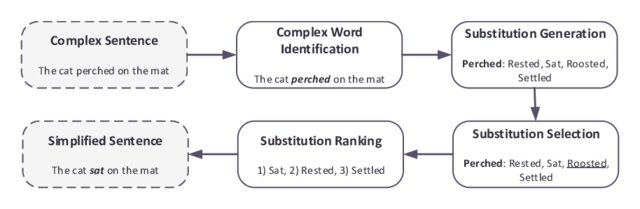
\includegraphics{img/lexical-simplification-pipeline.png}
	\caption{Afbeelding van \textcite{Althunayyan2021}}
	\label{img:pipeline-lexical-simplification}
\end{figure}

\begin{tabular}{ | m{4cm} | m{12cm} | } 
\hline
\textbf{Databank} & \textbf{Ondersteunde talen} \\
\hline
Engels & WordNet \\
& SWORDS \\
& LSBert \\
\hline
Nederlands & Celex \\
& NT2Lex \\
& Cornetto \\
\hline
Meertalig (Engels, Duits, Spaans en Portugees) & PHOR-in-One \\
\hline	
\caption{Beschikbare Nederlandstalige, Engelstalige en meertalige lexicale databanken anno mei 2023.}
\label{table:lexical-databases}
\end{tabular}

% gedaan door synoniemen te zoeken voor een doelwoord in lexicale databanken zoals WordNet, BERT, context2vec, nPIC of OOC. Uit een onderzoek van de Universiteit van KU Leuven stroomde een lexicale databank voor de Nederlandse taal verder voor, namelijk NT2Lex\footnote{https://cental.uclouvain.be/cefrlex/nt2lex/download/}.

\medspace

Om de complexiteit van een tekst te verminderen, kan syntactische vereenvoudiging worden toegepast door de grammatica en zinsstructuur aan te passen. Dit kan gedaan worden door het combineren van twee zinnen tot één eenvoudigere zin of door de syntax te vereenvoudigen, terwijl de inhoud behouden blijft. Een voorbeeld van zo'n model is ontwikkeld door \textcite{Kandula2010} voor medische informatie. Het model bestaat uit drie modules, die zinnen met meer dan tien woorden vereenvoudigen en eventueel vervangen door kortere zinnen. Het omvat een PoS Tagger, een Grammar Simplifier en een Output Validator als onderdelen van de architectuur.

\medspace

\begin{enumerate}
	\item Ten eerste wordt de PoS Tagger-functie uit het open-source pakket OpenNLP\footnote{https://opennlp.apache.org/} gebruikt.
	\item Vervolgens splitst de \textit{Grammar Simplifier}-module lange zinnen in kortere zinnen door middel van het identificeren van POS-patronen en het toepassen van transformatieregels.
	\item Tot slot controleert de \textit{Output Validator}-module de grammatica en leesbaarheid van de output van de Grammar Simplifier.
\end{enumerate}  

\medspace

Geautomatiseerde tekstvereenvoudiging is geen nieuw concept. Volgens onderzoeken van \textcite{Canning2000, Siddharthan2006} waren de eerste aanpakken op geautomatiseerde tekstvereenvoudiging gebouwd op rule-based modellen. Deze modellen bewerken de syntax door zinnen te splitsen, te verwijderen of de volgorde van de zinnen in een tekst aan te passen. Lexicale vereenvoudiging kwam hier niet aan de pas. Enkel bij recentere onderzoeken van \textcite{Coster2011, Bulte2018} werd het duidelijk hoe lexicale en syntactische vereenvoudiging gecombineerd kon worden.

\medspace

Vroegere onderzoeken tonen aan dat geautomatiseerde tekstvereenvoudiging al geruime tijd bestaat. Zo hebben \textcite{Canning2000} en \textcite{Siddharthan2006} onderzocht dat de eerste methoden gebaseerd waren op \textit{rule-based} modellen die de syntaxis van de tekst bewerken door zinnen te splitsen, te verwijderen of te herschikken. Lexicale vereenvoudiging speelde hierbij geen rol. Pas bij recentere onderzoeken, zoals die van \textcite{Coster2011} en \textcite{Bulte2018}, werd het duidelijk hoe lexicale en syntactische vereenvoudiging gecombineerd konden worden.

\medspace

Om wetenschappelijke artikelen toegankelijker en begrijpelijker te maken, is het van belang om de kernpunten van een artikel op een duidelijke en beknopte manier samen te vatten. Hoewel samenvatten niet gericht is op het vereenvoudigen van de tekst, is het wel een techniek die noodzakelijk is om de semantiek achter een tekst met zo min mogelijk woord- of tekens te kunnen begrijpen. Full-text-search en gepersonaliseerde informatiefiltering benadrukken het belang van deze op maat gemaakte samenvattingen. Een samenvattingssysteem bestaat uit drie fases: analyse van de brontekst, identificatie van de kernpunten en samenvoeging van deze kernpunten tot één overzichtelijke tekst. Het machinaal samenvatten van teksten is geen nieuw concept en kan op twee manieren worden gedaan: door extractie en door abstractie \autocite{Hahn2000, Dubay2004}.

\medspace

Bij het extraherend samenvatten van teksten worden de belangrijkste zinnen gemarkeerd en opnieuw geformuleerd. Dit kan echter leiden tot onsamenhangende uitvoertekst, zoals \textcite{Khan2014} heeft aangetoond. Om de kernzinnen te bepalen, kunnen verschillende methoden worden gebruikt, zoals woordfrequentie, zinpositie en gelijkenissen, de cue-methode, titels, de rest van het document, proper nouns, woordgebruik en de afstand tussen text units met entiteiten, aldus \textcite{Khan2014}. Verschillende technieken voor het extraherend samenvatten van teksten, waaronder graafgebaseerde methoden, maximal marginal relevance (MMR) en metaheuristiek-gebaseerde ES, zijn onderzocht door \textcite{Verma2020} en worden verder beschreven in Tabel \ref{table:extractive-summarization}.

\begin{center}
	\begin{tabular}{ | m{4cm} | m{12cm} | } 
		\hline
		MMR-gebaseerde ES & Deze traditionele techniek gebruikt de maximaal marginale relevantiescore (MMR) om de relevantie en diversiteit van gemarkeerde zinnen te bepalen. Zorgt ervoor dat de geselecteerde zinnen niet te veel overlappen in inhoud en relevantie. Kan leiden tot betere samenvattingen, maar vereist meer rekenkracht en tijd. \\
		\hline
		Graafgebaseerde ES & Deze techniek vertegenwoordigt een document als een graaf van zinnen en gebruikt algoritmen om de belangrijkste zinnen te bepalen en redundantie te vermijden. Kan zowel voor lange wetenschappelijke artikelen als korte nieuwsartikelen goede resultaten opleveren \autocite{McDonald2007, Lin2010}. \\ 
		\hline
		Metaheuristiek-gebaseerde ES & Deze techniek maakt gebruik van optimalisatie-algoritmen zoals genetische algoritmen en zwermoptimalisatie om de belangrijkste zinnen in een tekst te vinden \autocite{Premjith2015, Verma2020}. Evaluatiefunctie kan in een lokaal optimum vastlopen afhankelijk van de gebruikte criteria. \autocite{Rani2021}. \\
		\hline
	\end{tabular}
	\label{table:extractive-summarization}
\end{center}

\medspace

De extraherende samenvatting van nieuwsartikelen kan beïnvloed worden door de vooroordelen of \textit{bias} van de auteur, zo blijkt uit experimenten uitgevoerd door \textcite{McKeown1999}. Bij deze vorm van samenvatten worden de zinnen overgenomen zoals ze zijn. \textcite{Hahn2000} bouwde verder op deze experimenten door het combineren van \textit{knowledge-rich} en \textit{knowledge-poor} methoden, wat resulteerde in significante verbeteringen. Bij het extraherend samenvatten is het van belang om de meest relevante tekstgedeeltes te selecteren, meestal in de vorm van zinnen. Om de lexicale en statistische relevantie van een zin te kunnen bepalen, worden twee methoden genoemd door \textcite{Hahn2000}:

\begin{itemize}
	\item Het lineaire gewichtsmodel, waarbij elke teksteenheid wordt gewogen op basis van factoren zoals de positie van de zin en het aantal keren dat deze voorkomt.
	\item Het gewichtsmodel op basis van de statistische relevantie van een eenheid, waarbij rekening wordt gehouden met de aanwezigheid van woorden in (sub)titels.
\end{itemize}

\medspace

Om de nauwkeurigheid van modellen te verbeteren, hebben \textcite{Nallapati2017} \textit{SummaRuNNer} ontwikkeld: een oplossing voor het extraherend samenvatten van teksten met behulp van een neuraal netwerk. Het systeem is opgebouwd met \textit{PyTorch} en bestaat uit drie modellen: een recurrent neuraal netwerk, een convolutioneel recurrent neuraal netwerk en een hiërarchical attention network.

\medspace

Het ophalen van kernzinnen kan leiden tot een onsamenhangende tekst. Om samenhang te creëren tussen zinnen, worden kernzinnen vaak geparafraseerd in de taalwereld. Er zijn twee benaderingen om een tekst op een abstraherende manier samen te vatten: de semantisch-gebaseerde en de structuurgebaseerde benadering. De structuurgebaseerde methode gebruikt regels om belangrijke informatie in de tekst te vinden, maar kan leiden tot samengevatte zinnen met lage taalkundige kwaliteit en grammaticale fouten. De semantisch-gebaseerde benadering daarentegen gebruikt de betekenis van de tekst om korte en duidelijke samenvattingen te maken met minder redundante zinnen en betere taalkundige kwaliteit, hoewel een extra parsingfase nodig kan zijn. \textcite{Cao2022} deed verder onderzoek naar deep learning methoden om automatisch abstraherende samenvattingen te genereren. Deep learning-modellen zoals RNN's, CNN's en Seq2Seq kunnen worden gebruikt voor abstraherend samenvatten door de betekenis van de tekst te begrijpen en belangrijke informatie over te brengen \autocite{Suleiman2020}.

\medspace

Volgens \textcite{Hsu2018, Huang2019} zou een ideale samenvatting zowel abstraherend als extraherend moeten zijn. Een hybride samenvattings-pijplijn zou daarom twee fasen moeten bevatten: een \textit{content selection} fase waarin de kernzinnen worden opgehaald door middel van extraherende samenvatting, en een \textit{paraphrasing}-fase waarbij de gemarkeerde kernzinnen abstraherend worden samengevat.

\subsection{Ondersteunende en bevoordelende effecten van ATS voor scholieren met dyslexie}

% Uitleg over dit onderzoek

\begin{figure}[H]
	\begin{center}
		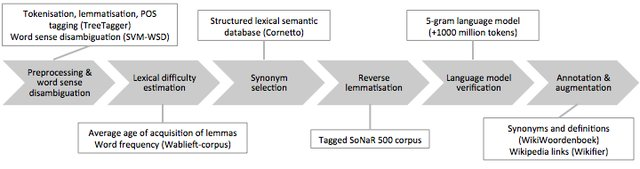
\includegraphics[width=9cm]{img/dutch-simplification-dyslexia-pipeline.png}
	\end{center}
	\caption{Afbeelding uit \textcite{Bulte2018}}
	\label{img:dyslexia-bulte-pipeline}
\end{figure}

\begin{figure}[H]
	\begin{center}
		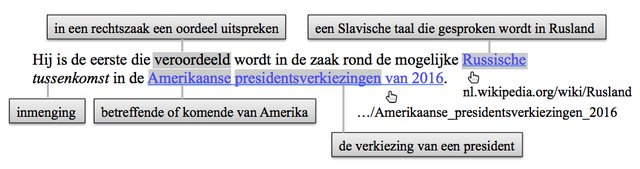
\includegraphics[width=9cm]{img/dutch-simplification-dyslexia-example.png}
	\end{center}
	\caption{Afbeelding uit \textcite{Bulte2018}}
	\label{img:dyslexia-bulte-example}
\end{figure}


Al zijn er onderzoeken over lexicale, syntactische en semantische vereenvoudiging voor kinderen en scholieren met dyslexie, het aantal onderzoeken over samenvatten voor deze doelgroep is schaars. Zoals eerder aangehaald is er wel onderzoek gedaan naar de verschillende manieren om een tekst samen te vatten, maar er is geen toepassing of onderzoek dat dit concreet uitwerkt. 

\subsection{MTS en ATS combineren}
% Hoe kunnen geautomatiseerde tekstvereenvoudiging en gepersonaliseerde tekstvereenvoudiging gecombineerd worden?

\textcite{Sanja2021} wijzen erop dat toepassingen voor tekstvereenvoudiging regelmatig als \textit{showcase} van de technologie ontwikkeld worden en zelden tot weinig rekening houden met personalisatieopties die nodig zijn om een vereenvoudiging op maat te kunnen genereren.

\medspace

Bij het ontwerpen van een ondersteunende toepassing voor dyslexie moet rekening worden gehouden met de individuele behoeften en uitdagingen van elke scholier, volgens \textcite{Gooding2022}. Dyslexie kan zich namelijk op verschillende manieren uiten bij verschillende scholieren, waarbij bijkomende symptomen niet altijd van invloed zijn op de spellingprestaties van een scholier. Om deze reden is het belangrijk om een toepassing te ontwerpen die rekening houdt met de diversiteit van dyslexie.

\subsection{Trends bij ATV}

% TODO LLM --> BERT / GPT-3

BERT is een meertalige Large Language Model (LLM) dat contextual word embeddings gebruikt. Het is getraind op 110 miljoen parameters uit 104 verschillende talen, waaronder Nederlands. Voor de Nederlandse taal zijn er twee varianten van BERT beschikbaar, namelijk RobBERT en BERTje. RobBERT wordt als krachtiger beschouwd. 

% TODO HuggingFace

\begin{tabular}{cols}
	content...
\end{tabular}

% TODO tabel

% Het is aangetoond in \textcite{Zhang2020} dat het Pegasus-model een pre-trained model gebruikt voor NLP-samenvatting en gap-zinnen afhandelt, en getraind en geëvalueerd is voor verschillende soorten samenvattings-taken. LED of Longformer Encoder-Decoder is specifiek ontworpen om lange documenten te verwerken, waardoor het geschikt is voor het samenvatten van lange wetenschappelijke artikelen. 

\section{Beschikbare tools en taalmodellen}

Dyslexie is een veelvoorkomende aandoening die de lees- en schrijfvaardigheden van scholieren kan belemmeren. Om deze scholieren te ondersteunen, worden er verschillende softwareprogramma's en tools ontwikkeld. In dit hoofdstuk zal worden gekeken naar mogelijke nationale en internationale software die specifiek is ontworpen om scholieren met dyslexie te helpen bij het lezen van teksten. Er zal met name worden gekeken naar de beschikbare software in Vlaamse middelbare scholen, chatbots, zoals Bing AI en ChatGPT, en software die speciaal is ontwikkeld om dyslexie te ondersteunen bij het lezen. Deze sectie beantwoordt de volgende onderzoeksvraag: "Welke toepassingen, tools en modellen zijn er beschikbaar om Nederlandstalige geautomatiseerde tekstvereenvoudiging met AI mogelijk te maken?"

\medspace

In het middelbaar onderwijs wordt lees- en studieondersteuning voor scholieren met dyslexie enkel in de vorm van voorleessoftware voorzien \autocite{DeCraemer2018, OnderwijsVlaanderen2023}. \textcite{OnderwijsVlaanderen2023} leent licenties voor de volgende softwarepakketten uit SprintPlus, Kurzweil3000, Alinea Suite, IntoWords en TextAid. Naast luister- en schrijfopties kunnen scholieren deze toepassingen gebruiken om zinnen te markeren om deze zinnen vervolgens samen te vatten. Enkel de gemarkeerde zinnen worden betrokken in de samengevatte versie, dus de zinnen blijven lexicaal, syntactisch en semantisch identiek. Alle vermelde softwarepakketten bieden echter geen onafhankelijke samenvat- of vereenvoudigfunctie aan. \textcite{Tops2018} benadrukt de handige aspecten van deze software, maar deze software moet zo vroeg mogelijk in een schoolcarriére worden ingezet. Zo raken de scholieren snel vertrouwd met het gebruik, wat kan leiden tot een optimaal gebruik in verdere studies. Volgens \textcite{Tops2018} is het te laat om deze software pas in het hoger onderwijs te introduceren.

\medspace

Online zijn er tools beschikbaar om teksten generiek samen te vatten. Resoomer, Paraphraser en Scholarcy zijn oorspronkelijk Engelstalige tools, met ondertussen de mogelijkheid om een abstraherende samenvatting te maken van Nederlandstalige teksten. Proof-of-concepts zijn in schaarse hoeveelheid beschikbaar. De taalmodellen waar deze applicaties op werken, is niet gekend. Daarnaast zijn er ook geen API's beschikbaar om mee te werken. Gepersonaliseerde toepassingen zijn er in mindere mate. \textcite{Bingel2018} omschrijft een proof-of-concept voor een webtoepassing dat teksten vereenvoudigd, met oog op mensen met dyslexie. Deze software noemt nu Hero en bevindt zich in betafase. Deze toepassing is ondertussen herwerkt als browserextensie bij selecte nieuwssites en kan daarmee niet gebruikt worden voor wetenschappelijke artikelen.

\medspace

Toepassingen om wetenschappelijke artikelen te vereenvoudigen zijn schaars, maar er zijn enkele gratis en betalende toepassingen beschikbaar. SciSpace\footnote{https://typeset.io/} is gratis. Scholarcy\footnote{https://www.scholarcy.com/?ref=theresanaiforthat} is betalend. 

\begin{figure}
	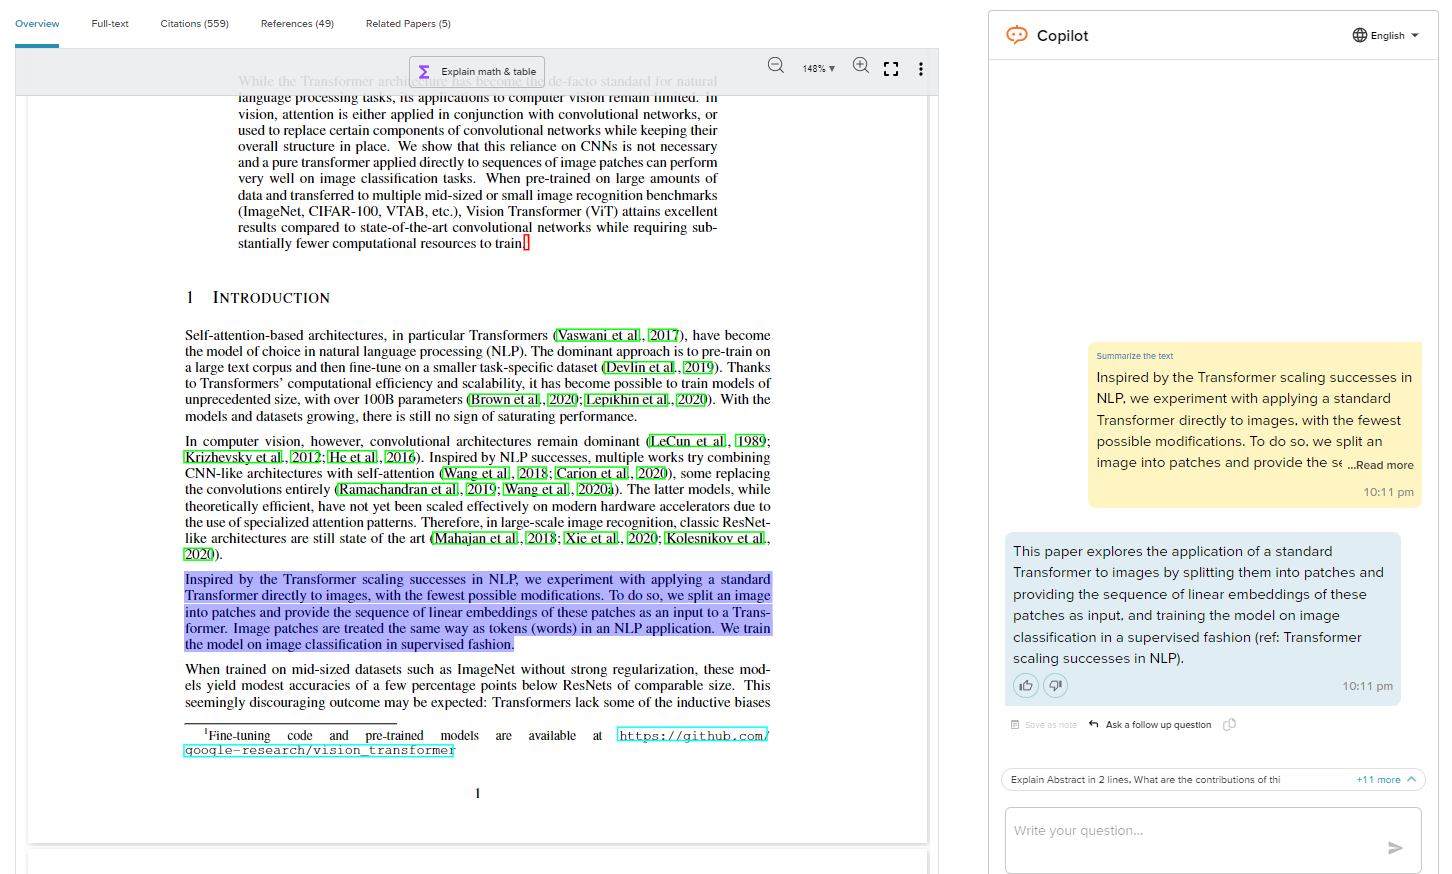
\includegraphics{img/typeset-example.png}
	\caption{Schermafbeelding van SciSpace}
\end{figure}

\medspace

\textit{Generative Pretrained Transformer 3} of GPT-3 is een taalmodel ontworpen door OpenAI. Dit taalmodel gebruikt een tweestapsleerparadigma waarbij het eerst ongesuperviseerd wordt getraind met een taalmodelleringsdoel en daarna gesuperviseerd wordt gefinetuned. Over drie versies heen is het model aanzienlijk vergroot, van anderhalf miljard parameters bij GPT-2 naar 175 miljard parameters bij GPT-3. Het model is getraind op niet-gecategoriseerde data van het internet en gebruikt datasets waaronder Common Crawl, WebText2, Books1, Books2, and Wikipedia \autocite{Radford2019, Li2022}.

\begin{itemize}
	\item In figuur \ref{img:simplification-gooding}: De invoertekst is een paragraaf uit een niet-vermeld boek van de Russische schrijver Dostoevsky. Het resultaat van de meegegeven prompt is een transformatie dat iedere vorm van vooraf aangehaalde vereenvoudiging weergeeft. Lexicale, conceptuele en syntactische vereenvoudiging worden op de invoertekst toegepast.
	\item In figuur \ref{img:different-versions-gooding}: Gooding haalt verder aan dat modellen zoals ChatGPT op twee vlakken de leesbaarheid van een tekst kan bevorderen. Allereerst door het verlenen van verschillende mogelijke versies van een vereenvoudigingstaak.
	\item In figuur \ref{img:evaluation-gooding}: ...
\end{itemize}

\begin{figure}[H]
	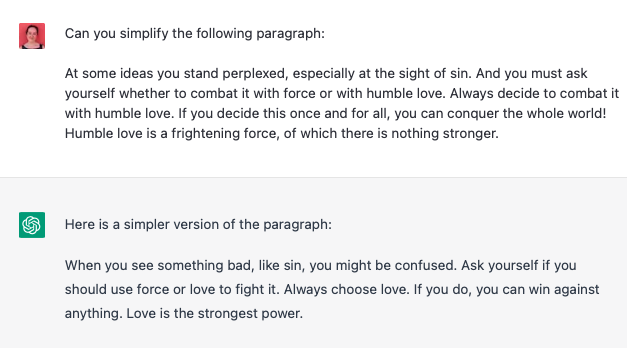
\includegraphics[width=10cm]{img/chatgpt-example-simplification-gooding.png}
	\caption{Afbeelding van Gooding 2022}
	\label{img:simplification-gooding}
\end{figure}

\begin{figure}[H]
	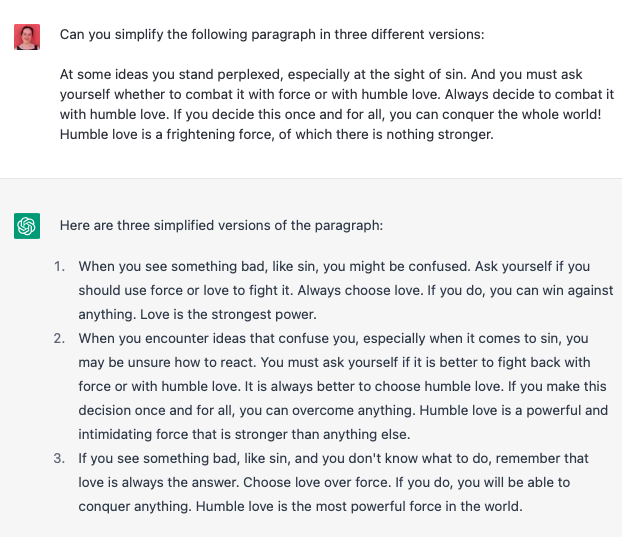
\includegraphics[width=10cm]{img/chatgpt-example-different-versions-gooding.png}
	\caption{Afbeelding van Gooding 2022}
	\label{img:different-versions-gooding}
\end{figure}

\begin{figure}[H]
	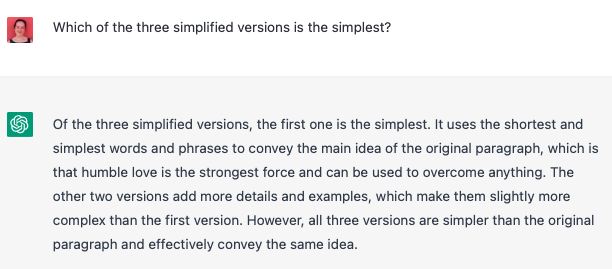
\includegraphics[width=10cm]{img/chatgpt-example-evaluation-gooding.png}
	\caption{Afbeelding van Gooding 2022.}
	\label{img:evaluation-gooding}
\end{figure}

\textcite{Lisowski2023} vergelijkt de twee OpenAI taalmodellen met een \textit{mixed-methods} onderzoek. Al blijken de twee heel gelijkaardig, het experiment benadrukt dat het ChatGPT-model gericht is op conversationele doeleinden met voorkeur als chatbot, terwijl GPT-3 een ML-model is bedoeld om met hoogstens één prompt te werken. De grootte van het GPT-3 model met 175 miljard parameters imposanter dan Chat-GPT. Daarnaast is de limiet bij het meest recente GPT-3 model is 4000 tokens. Verder haalt Lisowski aan dat de kwaliteit bij beide modellen sterk afhankelijk is van de invoer. De prompts moeten concreet genoeg zijn, om zo niet af te wijken van wat de gebruiker wilt \autocite{Lisowski2023}. Deze twee API's zijn nu vrij beschikbaar voor ontwikkelaars als betalende API \autocite{Brockman2023}.

\medspace

De documentatie van OpenAI\footnote{https://platform.openai.com/docs/} reikt vier verschillende engines voor het GPT-3 taalmodel aan, namelijk Davinci, Curie, Babbage en Ada. In Maart 2023 voegde een vijfde engine zich toe, namelijk GPT-3 Turbo wat de basis is achter Chat-GPT. Davinci-003 is het meest geavanceerde model dat alles kan wat de andere engines ook kunnen, met de meest menselijke antwoorden en geschikt voor taken zoals essays schrijven en code genereren. Curie is goed voor nuance maar minder menselijk dan Davinci, terwijl Ada en Babbage minder krachtig zijn en aangeraden worden voor eenvoudige taken zoals tekst aanvullen en sentiment analyse \autocite{Brockman2023}. Deze engines gebruiken eenzelfde set van hyperparameters die aangepast kunnen worden opgesomd in \ref{table:gpt-3-parameters}.

	\begin{tabular}{ m{3cm} | m{3cm} | m{10cm} | }
	\hline
	Parameter & Omschrijving & Mogelijke waarden \\
	\hline
	model & Het GPT-3 model om te gebruiken & davinci, curie, babbage, ada, text-davinci-002, text-curie-001, text-babbage-001, text-ada-001, davinci-codex \\
	\hline
	temperature & De gulzigheid van een generatief model. Een lagere waarde zal conservatieve en voorspelbare tekst teruggeven. Hogere waarden zullen meer gevarieerde en onverwachtse tekst teruggeven, wat beter werkt bij creatieve toepassingen. & Een kommagetal tussen 0 en 1. \\
	\hline
	max\_tokens & Het maximaal aantal tokens (woorden of subwoorden) dat het generatief model kan teruggeven. & Een getal tussen 1 and 2048. \\
	\hline
	top\_p & Vergelijkbaar met temperature, maar deze waarde onderhoudt de probability distribution voor common tokens. Hoe lager de waarde, hoe waarschijnlijker de woordenschat dat het model zal overwegen bij het genereren van tekst. Een hoge waarde is toepasselijker wanneer een toepassing gericht is op nauwkeurigheid en correctheid. & Een kommagetal tussen 0 en 1. \\
	\hline
	stop & Een tekstwaarde (woord/symbool) tot waar het model zal genereren. When the model generates a string that matches any of the specified strings, it stops generating text. & Een lijst van string-waarden, of een enkele string. \\
	\hline
	presence\_penalty & Factor die bepaalt hoe regelmatig woorden voorkomen. & Een kommagetal tussen 0 en 1 \\
	\hline
	\caption{Tabel met alle GPT-3 parameters.}
	\label{table:gpt-3-parameters}
\end{tabular}

\begin{figure}
	\begin{center}
		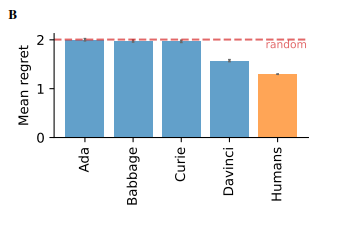
\includegraphics{img/chatgpt-engines-mean-regret.png}
		\caption{Afbeelding van \textcite{Binz2023}. Dit toont de \textit{mean regret} aan tussen de vier engines en de menselijke antwoorden.}
	\end{center}
\end{figure}

\medspace

De mogelijkheden van OpenAI's ChatGPT en GPT-3 modellen zijn nog volop in ontwikkeling, maar er zijn al enkele vergelijkende onderzoeken uitgevoerd. Uit het experiment van \textcite{Goyal2022} blijkt dat \textit{zero-shot} samenvattingen met GPT-3 beter presteren dan \textit{fine-tuned} modellen. Daarnaast haalt \textcite{Mottesi2023} verschillende tools aan die gebruik maken van de GPT-3 API, waaronder Jasper AI en ChatSonic. Ook voor het onderwijs zijn er mogelijkheden, zoals de hoge toegankelijkheid en granulaire personalisatie van het GPT-3 model \autocite{Roose2023, Garg2022}. Echter, GPT-3 is niet geschikt voor alle taken, zoals sentimentanalyse en -classificatie, waarvoor een kleinschaliger taalmodel beter presteert \autocite{Li2022}. Bovendien is er aandacht voor de ecologische effecten van de grote omvang van deze modellen, waarvoor alternatieve oplossingen zoals het gebruik van Cloud-infrastructuur en geschikte model finetuning worden voorgesteld \autocite{Strubell2019, Simon2021}.

\medspace

De architectuur tussen GPT-3 en BERT is volgens \textcite{Mottesi2023} het meest opvallende verschil. GPT-3 is een autoregressief model en houdt daarmee enkel rekening met de linkercontext bij het voorspellen of genereren van tekst. BERT daarentegen is bidirectioneel en neemt zowel de linker- als de rechtercontext in overweging. De bidirectionele werking is geschikt voor sentimentanalyse waarbij begrip van de volledige zincontext noodzakelijk is. GPT-3 heeft toegang tot meer informatie (45TB) dan BERT (3TB), wat het een voordeel kan geven tijdens taalbewerkingen waaronder het vereenvoudigen, parafraseren of het vertalen. Ten slotte verschillen de LLM's ook qua grootte. Hoewel beide modellen erg groot zijn, is GPT-3 aanzienlijk groter dan de voorganger mede door de uitgebreide trainingsdatasetgrootte \autocite{Brown2020}. LLaMa of Large Language Model Meta AI is een generatief taalmodel met potentieel dat sterker is dan GPT-3 en soortgelijke modellen, terwijl het van tien keer minder parameters gebruik maakt, maar is nog niet beschikbaar als online webtoepassing of API \autocite{Hern2023, Touvron2023}.


\begin{figure}[H]
	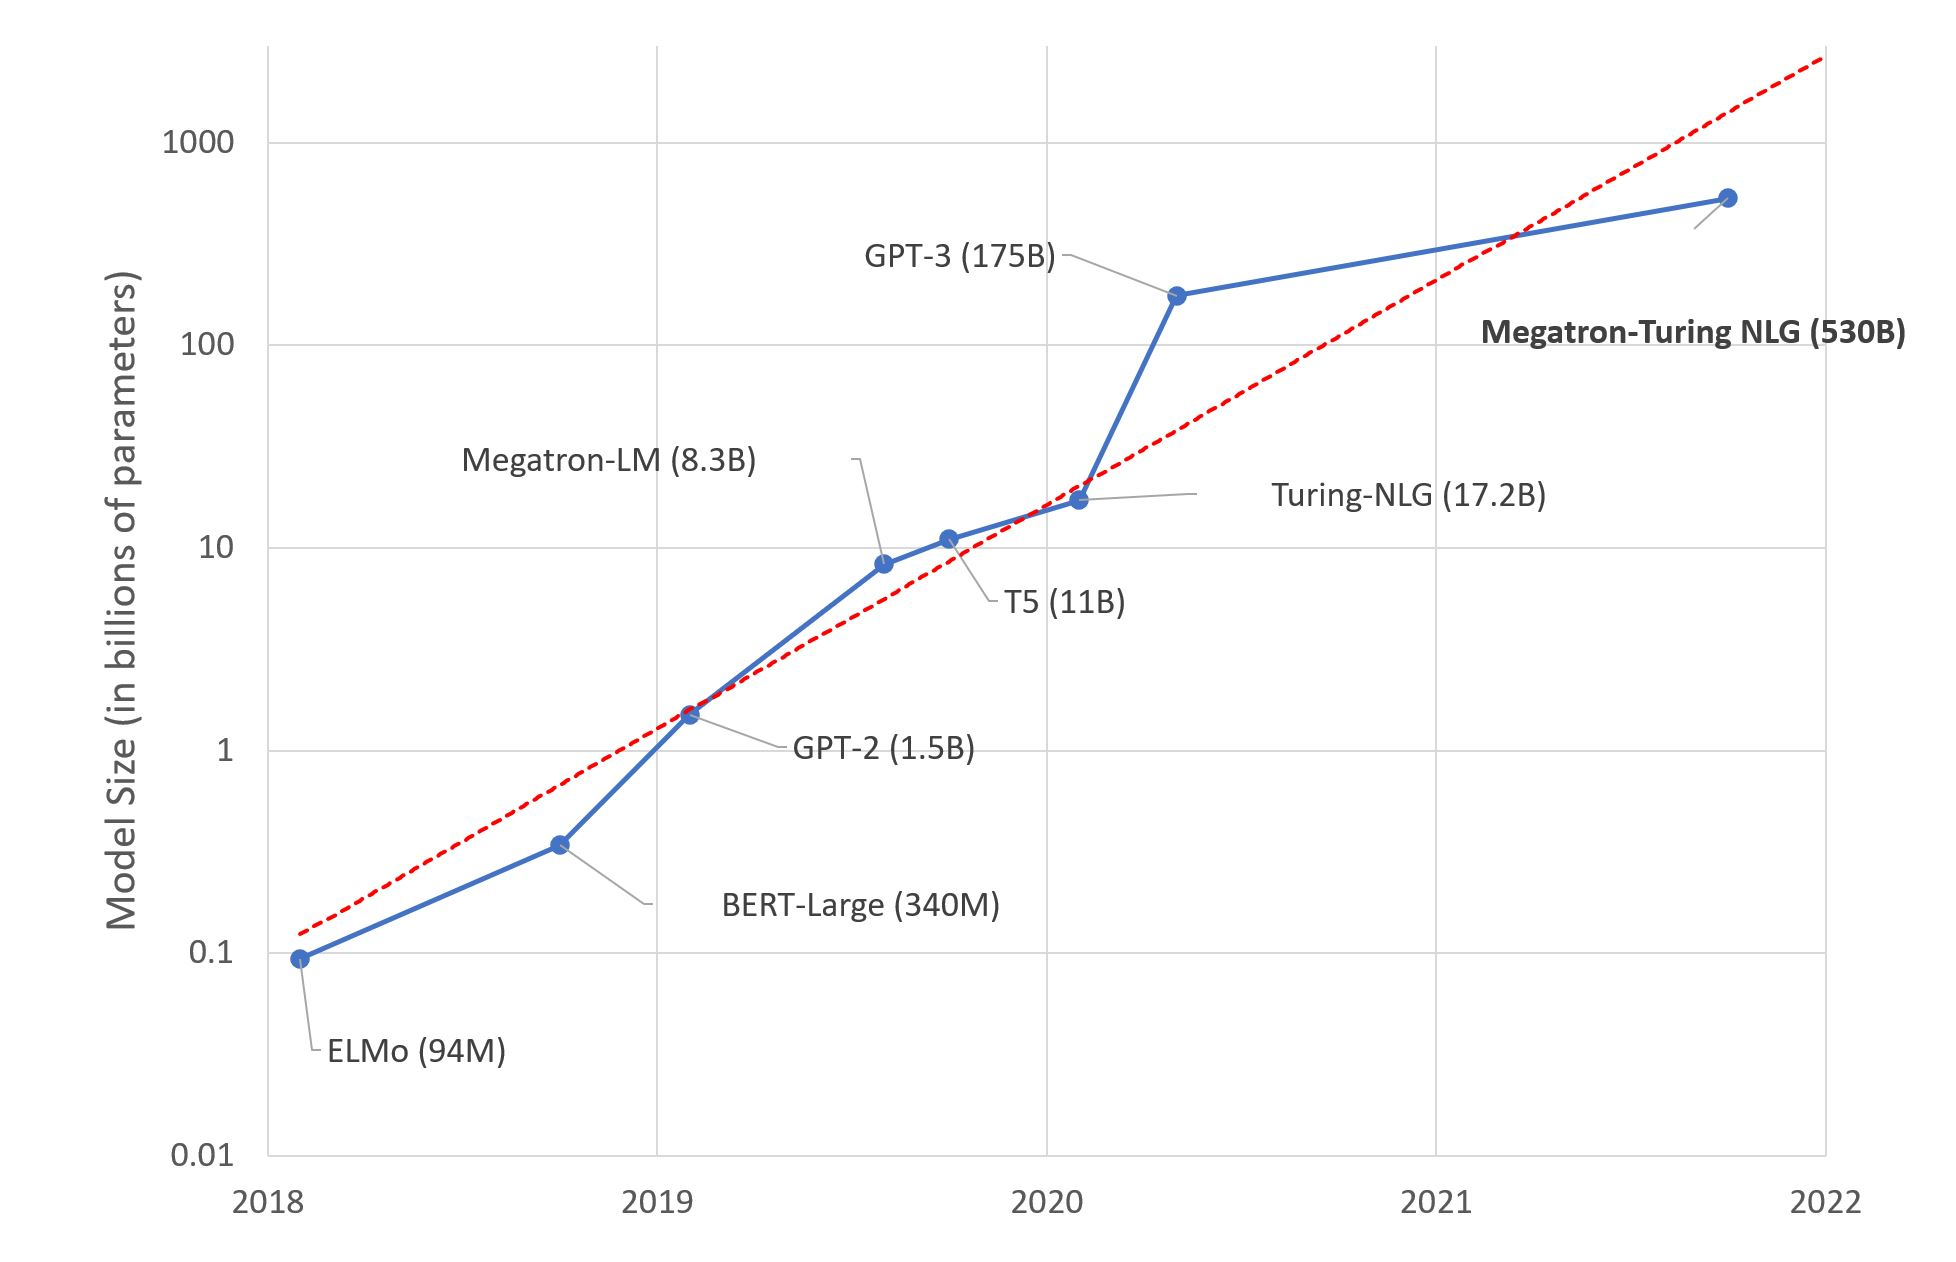
\includegraphics{img/graph-language-models.png}
	\caption{Afbeelding van \textcite{Simon2021}. De evolutie van pre-trained taalmodellen wordt hier weergegeven tot eind 2022. De performantie van de modellen ten opzichte van de grootte volgt een lineaire functie.}
\end{figure}

\medspace

Microsoft en OpenAI werken nauw samen. Zo maakt het conversationele taalmodel van Bing ook gebruik van GPT-3. Deze chatbot bouwt verder en biedt zo verwijzingen en referenties aan naar andere websites. Deze verwijzingen zijn volgens mogelijk door de Prometheus-technologie van Microsoft \autocite{Ribas2023}. Prometheus is een eigen technologie die door Bing is ontwikkeld. Het AI-model is volgens \textcite{Ribas2023} de eerste van zijn soort die de Bing-index-, ranking- en antwoordresultaten combineert met het redeneervermogen van OpenAI’s GPT-modellen. Prometheus maakt gebruik van de kracht van Bing en GPT om iteratief via een component genaamd \textit{Bing Orchestrator} een set interne queries te genereren met als doel binnen gegeven gesprekscontext een nauwkeurig antwoord op gebruikersqueries te bieden \autocite{Ribas2023}. Bing AI is nu in testfase met wachtlijst en bestaat in de vorm van een webpagina en een browserextensie voor Microsoft Edge. Onderzoek naar deze chatbot staat nog in de kinderschoenen en er is nood aan onderzoek naar de credibiliteit en correctheid van de verwijzingen. Deze chatbot gebruikt een combinatie van extraherende en abstraherende samenvattingen. In tegenstelling tot GPT-3 is er geen officiële API beschikbaar. Daarnaast is de limiet ook lager met 2000 tokens per bericht tijdens een conversatie. 

\begin{figure}[H]
	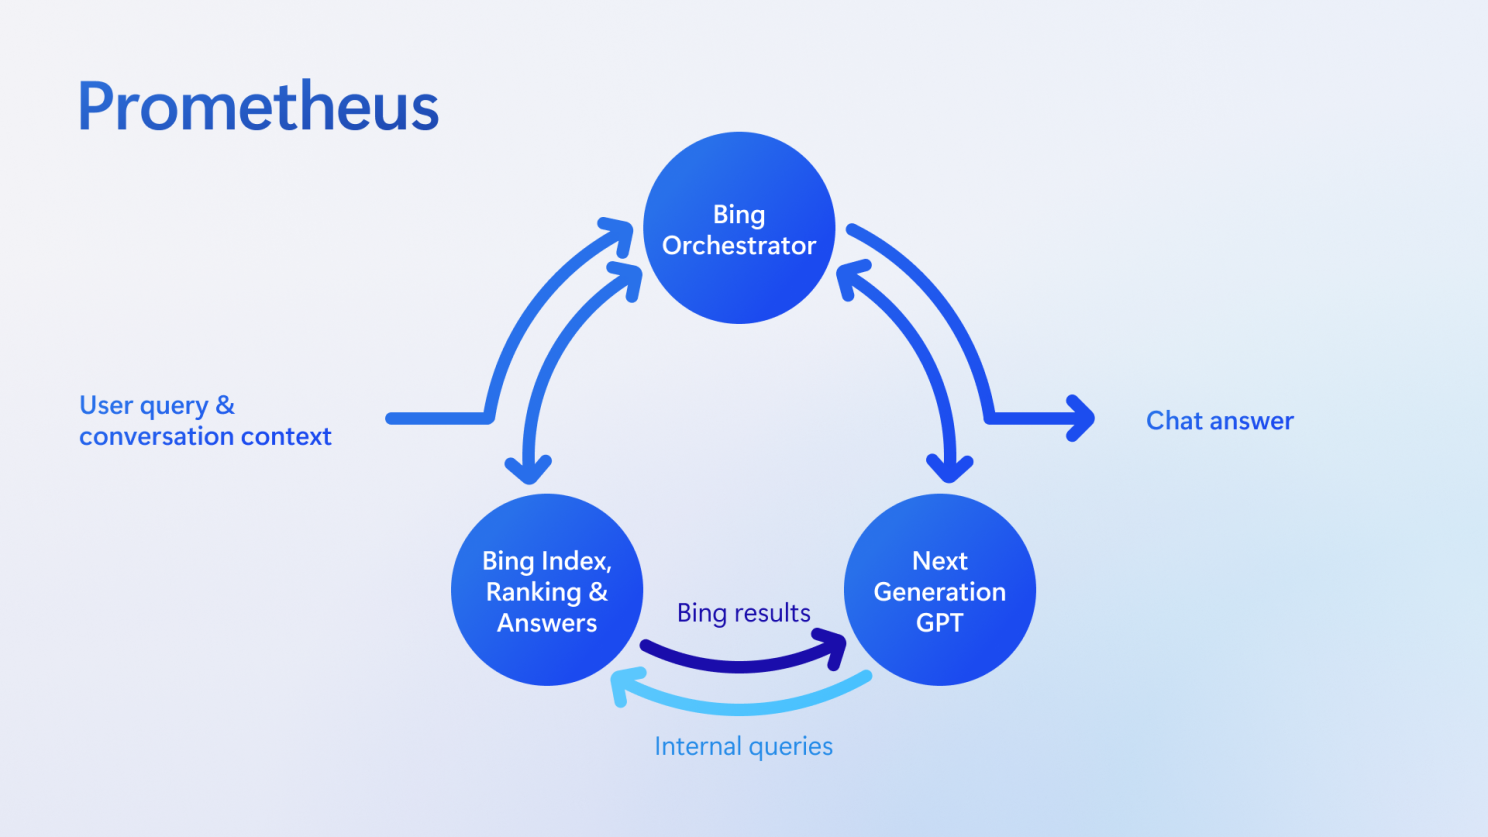
\includegraphics[width=6cm]{img/bing-ai-prometheus.png}
	\caption{Afbeelding van \textcite{Ribas2023}.}
\end{figure}

\begin{figure}[H]
	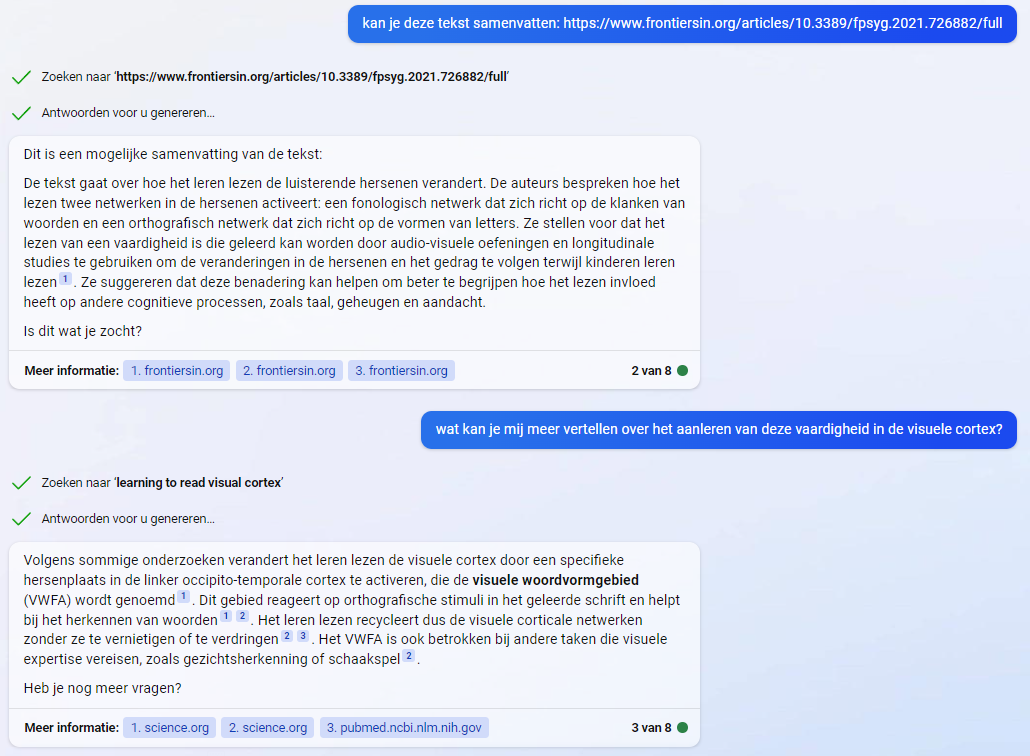
\includegraphics{img/bing-ai-chatbot-example.png}
	\caption{In deze afbeelding wordt er een online wetenschappelijk artikel meegegeven. Er wordt geen titel of onderwerp meegegeven, maar de Bing AI chatbot is in staat om een abstraherende samenvatting te maken van het artikel. Daarna geeft de chatbot verder uitleg over een bepaald onderwerp en geeft het extra referenties mee.}
\end{figure}

\medspace

In recente literatuur is Huggingface beschreven als een platform of portaalsite voor het delen van ML-modellen en datasets. De bibliotheek biedt een scala aan API's en tools die gemakkelijk te downloaden en trainen zijn voor pretrained modellen voor prevalente NLP-taken, zoals tekstclassificatie, taalmodellering en samenvatting. Deze modellen kunnen worden gefinetuned op specifieke datasets, waardoor ontwikkelaars snel modellen kunnen bouwen en inzetten voor vereenvoudigings- en samenvattingstaken. Voor wetenschappelijke documenten en artikelen bestaan er al enkele modellen en datasets: \footnote{https://huggingface.co/sambydlo/bart-large-scientific-lay-summarisation}, \footnote{https://huggingface.co/haining/scientific\_abstract\_simplification}

\subsection{Conclusie}

Experten halen het GPT-3 model en ChatGPT aan als de toekomst voor gepersonaliseerde en adaptieve uitleg aan scholieren. Bing AI biedt een extra dat revolutionair kan zijn bij het opzoeken van uitleg voor zoektermen, zonder het verlies aan bronvermelding. Huidige toepassingen staan mogelijks in een spreekwoordelijke schaduw eenmaal leessoftware voor scholieren met dyslexie worden ontwikkeld met AI. De mogelijkheden van GPT-3 zijn eindeloos en toepassingen die hiervan gebruik maken, kunnen in het onderwijs ingezet worden als ondersteunende software.


\section{De valkuilen bij AI en NLP.}
% 3 Met welke valkuilen bij taalverwerking met AI moeten ontwikkelaars rekening houden?
AI en ML zijn volop in groei. NLP gebruikt AI en ML om menselijke taal te verwerken, terwijl NLU deze technologieën gebruikt om menselijke taal te begrijpen. Hoewel deze technologieën veelbelovend zijn, moeten AI-ontwikkelaars rekening houden met veelvoorkomende en genegligeerde uitdagingen en valkuilen \autocite{Sciforce2020, Roldos2020, Khurana2022}. Deze sectie beantwoordt de volgende onderzoeksvraag: "Met welke valkuilen bij taalverwerking met AI moeten ontwikkelaars rekening houden?"

\medspace

NLP- en NLU-toepassingen behoren tot de duurste om te ontwikkelen, wat een obstakel kan vormen voor veel IT-professionals. Het gebrek aan NLP-expertise, de kwaliteit en kwantiteit van data, de integratie en deployment van modellen en de transparantie van modellen zijn allemaal factoren die bijdragen aan deze hoge kosten \autocite{IBM2022}. Software-ontwikkelaars verkiezen volgens  voor \textit{black-box} modellen bij de ontwikkeling en finetuning van een NLP-toepassing met AI. Al is het verschil qua nauwkeurigheid minimaal, de afweging wordt gemaakt bij de transparantie van het model. Na een transformatie wordt er niet aangegeven waarom specifieke transformaties werden uitgevoerd, bijvoorbeeld het vervangen van een woord door een eenvoudiger synoniem. White-box taalmodellen zijn er in schaarse hoeveelheden \autocite{Punardeep2020}.

\medspace 

Homoniemen kunnen volgens \textcite{Roldos2020} problemen veroorzaken bij sequence labeling of het labelen van tokens in een doorlopende tekst. Bijvoorbeeld bij het woord ‘bank’ is het niet duidelijk voor de machine of het gaat over de geldinstelling of het meubel. Word Sense Disambiguation (WSD), PoS-tagging en contextual embeddings kunnen de betekenis van een woord achterhalen op basis van de context \autocite{Eisenstein2019, Liu2020}. Het gebruik van synoniemen en antoniemen in NLP-systemen kan verbeterd worden door het gebruik van candidate generation en synonym detection, en meertalige transformers zoals BERT bieden een oplossing voor het gebrek aan niet-Engelstalige toepassingen \autocite{Dandekar2016, Roldos2020}.

\medspace

Tekstvereenvoudiging is bedoeld om gelijke kansen te bieden aan iedereen, maar ethische overwegingen en bewustzijn van de behoeften van de eindgebruiker zijn belangrijk bij het ontwikkelen van adaptieve tekstvereenvoudigingstoepassingen, zoals beschreven in onderzoeken van \textcite{Niemeijer2010, Xu2015, Gooding2022}. De eindgebruiker moet de keuze hebben om te kiezen welke delen van de tekst vereenvoudigd moeten worden, wat kan worden bereikt door synoniemen te kiezen of zinnen te markeren die moeilijk te begrijpen zijn.

\medspace

Iedereen kan converseren met een chatbot, maar de gepaste en verwachte antwoorden krijgen vergt een doordachte input. Een onnauwkeurige prompt of gebrek aan trainingsdata kan leiden tot onjuiste output, terwijl het gebruik van conditionele expressies of finetunen van hyperparameters kan helpen de betrouwbaarheid van het antwoord te vergroten \autocite{Miszczak2023, Jiang2023}.

\medspace

Vergeleken met andere ML- of NLP-taken vergt het beoordelen van een vereenvoudigde tekst voldoende aandacht en opvolging van de ontwikkelaar. Evaluatiemetrieken zoals ROUGE en BLEU zijn beperkt, omdat ze geen rekening houden met de semantiek tussen een referentietekst en een vereenvoudigde tekst. Als valnet kunnen ontwikkelaars menselijk evaluatie inschakelen om de vereenvoudigde tekst van een taalmodel te beoordelen volgens \textcite{Fabbri2020}. De onderzoekers stimuleren verder onderzoek naar nieuwe standaarden en \textit{best practices} voor betrouwbare menselijke beoordeling. De doelgroep waarvoor een tekst wordt vereenvoudigd, moeten nauw in het proces worden opgenomen \autocite{Iskender2021}.


\section{Conclusie}

De noden van scholieren met fonologische dyslexie in de derde graad van het middelbaar gaan verder dan gewoon moeizaam lezen.  Het ontcijferen en automatiseren van woordeherkenning gebeurt langzaam. Er zijn bewezen voordelen van MTV en aangepaste visuele weergaven op kinderen en jongeren met dyslexie. De leesbaarheid van wetenschappelijke artikelen bevindt zich in een dalende trend. Het formaat, gebruik van vakjargon en ingewikkelde woordenschat en ten slotte de moeizame syntax en zinsbouw sluiten een algemene doelgroep uit bij het lezen van wetenschappelijke artikelen. Enkel wetenschappelijk geletterden zijn in staat om deze artikelen te lezen. Het uniforme formaat van een wetenschappelijk artikel biedt kansen aan voor een geautomatiseerde aanpak tot het vereenvoudigen van een tekst.

\medspace

Experten halen meerdere bewezen tactieken aan om teksten automatisch te vereenvoudigen op maat voor een scholier met dyslexie. Handmatig worden teksten vereenvoudigd aan de hand van leesbaarheidsformules of intuïtie. Zinnen moeten lexicaal, syntactisch en semantisch worden vereenvoudigd. Teksten samenvatten maakt de tekst korter zonder het verlies van de kernboodschap. Voor deze vier transformaties zijn er taalmodellen beschikbaar in de vorm van API's of open-source software. Huidige software dat de overheid uitleent aan scholieren met dyslexie in het middelbaar onderwijs fungeert voornamelijk als voorleessoftware. Nieuwe en opkomende technologieën en taalmodellen zoals GPT-3 blinken uit om tekstvereenvoudiging mogelijk te maken. De ontwikkeling met LLM's is in opmars, maar ontwikkelaars moeten bewust zijn dat andere taalmodellen zoals BERT voor taken zoals semantische analyse minder rekenkracht vereisen voor eenzelfde en soms beter resultaat. 